% Created by tikzDevice version 0.12.3 on 2020-05-27 21:27:55
% !TEX encoding = UTF-8 Unicode
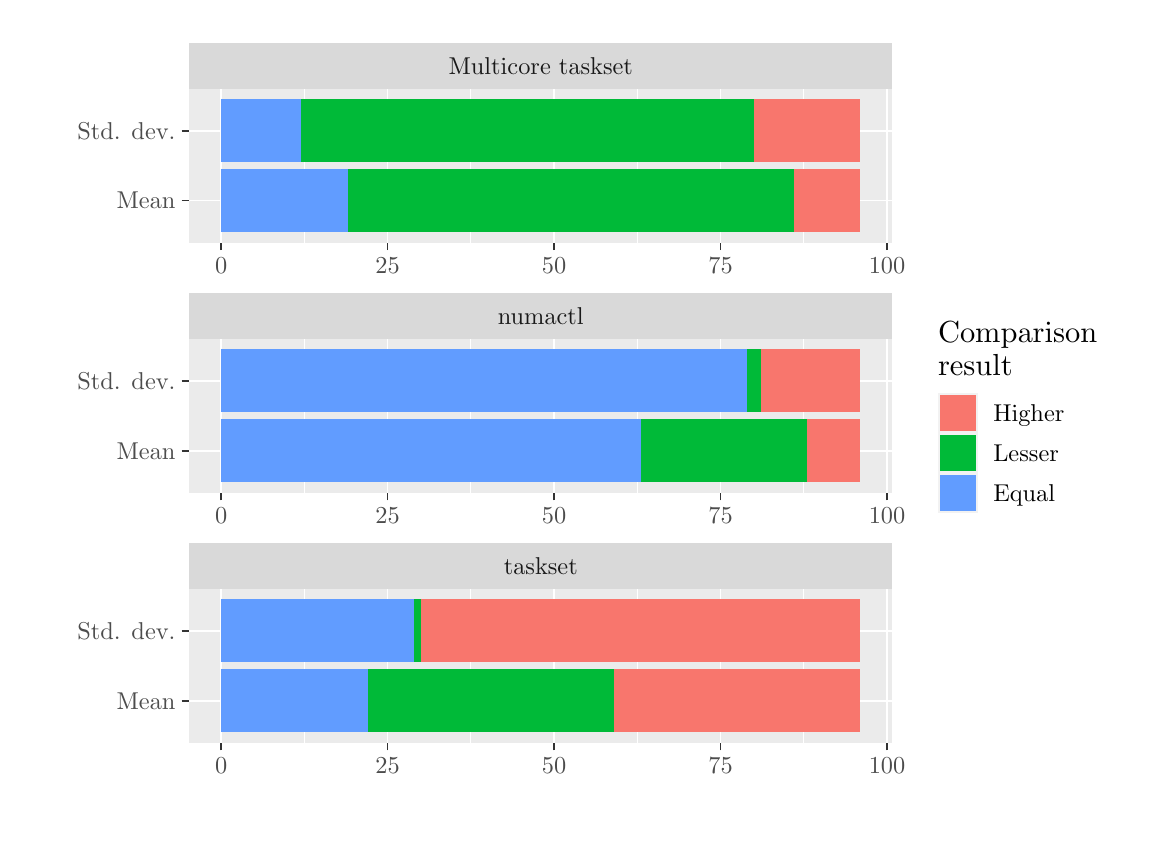
\begin{tikzpicture}[x=1pt,y=1pt]
\definecolor{fillColor}{RGB}{255,255,255}
\path[use as bounding box,fill=fillColor,fill opacity=0.00] (0,0) rectangle (397.48,289.08);
\begin{scope}
\path[clip] (  0.00,  0.00) rectangle (397.48,289.08);
\definecolor{drawColor}{RGB}{255,255,255}
\definecolor{fillColor}{RGB}{255,255,255}

\path[draw=drawColor,line width= 0.6pt,line join=round,line cap=round,fill=fillColor] (  0.00,  0.00) rectangle (397.48,289.08);
\end{scope}
\begin{scope}
\path[clip] ( 58.35,211.43) rectangle (312.46,267.01);
\definecolor{fillColor}{gray}{0.92}

\path[fill=fillColor] ( 58.35,211.43) rectangle (312.46,267.01);
\definecolor{drawColor}{RGB}{255,255,255}

\path[draw=drawColor,line width= 0.3pt,line join=round] ( 99.98,211.43) --
	( 99.98,267.01);

\path[draw=drawColor,line width= 0.3pt,line join=round] (160.14,211.43) --
	(160.14,267.01);

\path[draw=drawColor,line width= 0.3pt,line join=round] (220.30,211.43) --
	(220.30,267.01);

\path[draw=drawColor,line width= 0.3pt,line join=round] (280.46,211.43) --
	(280.46,267.01);

\path[draw=drawColor,line width= 0.6pt,line join=round] ( 58.35,226.59) --
	(312.46,226.59);

\path[draw=drawColor,line width= 0.6pt,line join=round] ( 58.35,251.85) --
	(312.46,251.85);

\path[draw=drawColor,line width= 0.6pt,line join=round] ( 69.90,211.43) --
	( 69.90,267.01);

\path[draw=drawColor,line width= 0.6pt,line join=round] (130.06,211.43) --
	(130.06,267.01);

\path[draw=drawColor,line width= 0.6pt,line join=round] (190.22,211.43) --
	(190.22,267.01);

\path[draw=drawColor,line width= 0.6pt,line join=round] (250.38,211.43) --
	(250.38,267.01);

\path[draw=drawColor,line width= 0.6pt,line join=round] (310.54,211.43) --
	(310.54,267.01);
\definecolor{fillColor}{RGB}{248,118,109}

\path[fill=fillColor] (276.85,215.22) rectangle (300.91,237.96);
\definecolor{fillColor}{RGB}{0,186,56}

\path[fill=fillColor] (115.62,215.22) rectangle (276.85,237.96);
\definecolor{fillColor}{RGB}{97,156,255}

\path[fill=fillColor] ( 69.90,215.22) rectangle (115.62,237.96);
\definecolor{fillColor}{RGB}{248,118,109}

\path[fill=fillColor] (262.41,240.48) rectangle (300.91,263.22);
\definecolor{fillColor}{RGB}{0,186,56}

\path[fill=fillColor] ( 98.78,240.48) rectangle (262.41,263.22);
\definecolor{fillColor}{RGB}{97,156,255}

\path[fill=fillColor] ( 69.90,240.48) rectangle ( 98.78,263.22);
\end{scope}
\begin{scope}
\path[clip] ( 58.35,121.06) rectangle (312.46,176.64);
\definecolor{fillColor}{gray}{0.92}

\path[fill=fillColor] ( 58.35,121.06) rectangle (312.46,176.64);
\definecolor{drawColor}{RGB}{255,255,255}

\path[draw=drawColor,line width= 0.3pt,line join=round] ( 99.98,121.06) --
	( 99.98,176.64);

\path[draw=drawColor,line width= 0.3pt,line join=round] (160.14,121.06) --
	(160.14,176.64);

\path[draw=drawColor,line width= 0.3pt,line join=round] (220.30,121.06) --
	(220.30,176.64);

\path[draw=drawColor,line width= 0.3pt,line join=round] (280.46,121.06) --
	(280.46,176.64);

\path[draw=drawColor,line width= 0.6pt,line join=round] ( 58.35,136.22) --
	(312.46,136.22);

\path[draw=drawColor,line width= 0.6pt,line join=round] ( 58.35,161.48) --
	(312.46,161.48);

\path[draw=drawColor,line width= 0.6pt,line join=round] ( 69.90,121.06) --
	( 69.90,176.64);

\path[draw=drawColor,line width= 0.6pt,line join=round] (130.06,121.06) --
	(130.06,176.64);

\path[draw=drawColor,line width= 0.6pt,line join=round] (190.22,121.06) --
	(190.22,176.64);

\path[draw=drawColor,line width= 0.6pt,line join=round] (250.38,121.06) --
	(250.38,176.64);

\path[draw=drawColor,line width= 0.6pt,line join=round] (310.54,121.06) --
	(310.54,176.64);
\definecolor{fillColor}{RGB}{248,118,109}

\path[fill=fillColor] (281.66,124.85) rectangle (300.91,147.58);
\definecolor{fillColor}{RGB}{0,186,56}

\path[fill=fillColor] (221.50,124.85) rectangle (281.66,147.58);
\definecolor{fillColor}{RGB}{97,156,255}

\path[fill=fillColor] ( 69.90,124.85) rectangle (221.50,147.58);
\definecolor{fillColor}{RGB}{248,118,109}

\path[fill=fillColor] (264.82,150.11) rectangle (300.91,172.85);
\definecolor{fillColor}{RGB}{0,186,56}

\path[fill=fillColor] (260.00,150.11) rectangle (264.82,172.85);
\definecolor{fillColor}{RGB}{97,156,255}

\path[fill=fillColor] ( 69.90,150.11) rectangle (260.00,172.85);
\end{scope}
\begin{scope}
\path[clip] ( 58.35, 30.69) rectangle (312.46, 86.26);
\definecolor{fillColor}{gray}{0.92}

\path[fill=fillColor] ( 58.35, 30.69) rectangle (312.46, 86.26);
\definecolor{drawColor}{RGB}{255,255,255}

\path[draw=drawColor,line width= 0.3pt,line join=round] ( 99.98, 30.69) --
	( 99.98, 86.26);

\path[draw=drawColor,line width= 0.3pt,line join=round] (160.14, 30.69) --
	(160.14, 86.26);

\path[draw=drawColor,line width= 0.3pt,line join=round] (220.30, 30.69) --
	(220.30, 86.26);

\path[draw=drawColor,line width= 0.3pt,line join=round] (280.46, 30.69) --
	(280.46, 86.26);

\path[draw=drawColor,line width= 0.6pt,line join=round] ( 58.35, 45.84) --
	(312.46, 45.84);

\path[draw=drawColor,line width= 0.6pt,line join=round] ( 58.35, 71.11) --
	(312.46, 71.11);

\path[draw=drawColor,line width= 0.6pt,line join=round] ( 69.90, 30.69) --
	( 69.90, 86.26);

\path[draw=drawColor,line width= 0.6pt,line join=round] (130.06, 30.69) --
	(130.06, 86.26);

\path[draw=drawColor,line width= 0.6pt,line join=round] (190.22, 30.69) --
	(190.22, 86.26);

\path[draw=drawColor,line width= 0.6pt,line join=round] (250.38, 30.69) --
	(250.38, 86.26);

\path[draw=drawColor,line width= 0.6pt,line join=round] (310.54, 30.69) --
	(310.54, 86.26);
\definecolor{fillColor}{RGB}{248,118,109}

\path[fill=fillColor] (211.88, 34.48) rectangle (300.91, 57.21);
\definecolor{fillColor}{RGB}{0,186,56}

\path[fill=fillColor] (122.84, 34.48) rectangle (211.88, 57.21);
\definecolor{fillColor}{RGB}{97,156,255}

\path[fill=fillColor] ( 69.90, 34.48) rectangle (122.84, 57.21);
\definecolor{fillColor}{RGB}{248,118,109}

\path[fill=fillColor] (142.09, 59.74) rectangle (300.91, 82.48);
\definecolor{fillColor}{RGB}{0,186,56}

\path[fill=fillColor] (139.69, 59.74) rectangle (142.09, 82.48);
\definecolor{fillColor}{RGB}{97,156,255}

\path[fill=fillColor] ( 69.90, 59.74) rectangle (139.69, 82.48);
\end{scope}
\begin{scope}
\path[clip] ( 58.35, 86.26) rectangle (312.46,102.84);
\definecolor{fillColor}{gray}{0.85}

\path[fill=fillColor] ( 58.35, 86.26) rectangle (312.46,102.84);
\definecolor{drawColor}{gray}{0.10}

\node[text=drawColor,anchor=base,inner sep=0pt, outer sep=0pt, scale=  0.88] at (185.41, 91.52) {taskset};
\end{scope}
\begin{scope}
\path[clip] ( 58.35,176.64) rectangle (312.46,193.21);
\definecolor{fillColor}{gray}{0.85}

\path[fill=fillColor] ( 58.35,176.64) rectangle (312.46,193.21);
\definecolor{drawColor}{gray}{0.10}

\node[text=drawColor,anchor=base,inner sep=0pt, outer sep=0pt, scale=  0.88] at (185.41,181.89) {numactl};
\end{scope}
\begin{scope}
\path[clip] ( 58.35,267.01) rectangle (312.46,283.58);
\definecolor{fillColor}{gray}{0.85}

\path[fill=fillColor] ( 58.35,267.01) rectangle (312.46,283.58);
\definecolor{drawColor}{gray}{0.10}

\node[text=drawColor,anchor=base,inner sep=0pt, outer sep=0pt, scale=  0.88] at (185.41,272.26) {Multicore taskset};
\end{scope}
\begin{scope}
\path[clip] (  0.00,  0.00) rectangle (397.48,289.08);
\definecolor{drawColor}{gray}{0.20}

\path[draw=drawColor,line width= 0.6pt,line join=round] ( 69.90, 27.94) --
	( 69.90, 30.69);

\path[draw=drawColor,line width= 0.6pt,line join=round] (130.06, 27.94) --
	(130.06, 30.69);

\path[draw=drawColor,line width= 0.6pt,line join=round] (190.22, 27.94) --
	(190.22, 30.69);

\path[draw=drawColor,line width= 0.6pt,line join=round] (250.38, 27.94) --
	(250.38, 30.69);

\path[draw=drawColor,line width= 0.6pt,line join=round] (310.54, 27.94) --
	(310.54, 30.69);
\end{scope}
\begin{scope}
\path[clip] (  0.00,  0.00) rectangle (397.48,289.08);
\definecolor{drawColor}{gray}{0.30}

\node[text=drawColor,anchor=base,inner sep=0pt, outer sep=0pt, scale=  0.88] at ( 69.90, 19.68) {0};

\node[text=drawColor,anchor=base,inner sep=0pt, outer sep=0pt, scale=  0.88] at (130.06, 19.68) {25};

\node[text=drawColor,anchor=base,inner sep=0pt, outer sep=0pt, scale=  0.88] at (190.22, 19.68) {50};

\node[text=drawColor,anchor=base,inner sep=0pt, outer sep=0pt, scale=  0.88] at (250.38, 19.68) {75};

\node[text=drawColor,anchor=base,inner sep=0pt, outer sep=0pt, scale=  0.88] at (310.54, 19.68) {100};
\end{scope}
\begin{scope}
\path[clip] (  0.00,  0.00) rectangle (397.48,289.08);
\definecolor{drawColor}{gray}{0.20}

\path[draw=drawColor,line width= 0.6pt,line join=round] ( 69.90,118.31) --
	( 69.90,121.06);

\path[draw=drawColor,line width= 0.6pt,line join=round] (130.06,118.31) --
	(130.06,121.06);

\path[draw=drawColor,line width= 0.6pt,line join=round] (190.22,118.31) --
	(190.22,121.06);

\path[draw=drawColor,line width= 0.6pt,line join=round] (250.38,118.31) --
	(250.38,121.06);

\path[draw=drawColor,line width= 0.6pt,line join=round] (310.54,118.31) --
	(310.54,121.06);
\end{scope}
\begin{scope}
\path[clip] (  0.00,  0.00) rectangle (397.48,289.08);
\definecolor{drawColor}{gray}{0.30}

\node[text=drawColor,anchor=base,inner sep=0pt, outer sep=0pt, scale=  0.88] at ( 69.90,110.05) {0};

\node[text=drawColor,anchor=base,inner sep=0pt, outer sep=0pt, scale=  0.88] at (130.06,110.05) {25};

\node[text=drawColor,anchor=base,inner sep=0pt, outer sep=0pt, scale=  0.88] at (190.22,110.05) {50};

\node[text=drawColor,anchor=base,inner sep=0pt, outer sep=0pt, scale=  0.88] at (250.38,110.05) {75};

\node[text=drawColor,anchor=base,inner sep=0pt, outer sep=0pt, scale=  0.88] at (310.54,110.05) {100};
\end{scope}
\begin{scope}
\path[clip] (  0.00,  0.00) rectangle (397.48,289.08);
\definecolor{drawColor}{gray}{0.20}

\path[draw=drawColor,line width= 0.6pt,line join=round] ( 69.90,208.68) --
	( 69.90,211.43);

\path[draw=drawColor,line width= 0.6pt,line join=round] (130.06,208.68) --
	(130.06,211.43);

\path[draw=drawColor,line width= 0.6pt,line join=round] (190.22,208.68) --
	(190.22,211.43);

\path[draw=drawColor,line width= 0.6pt,line join=round] (250.38,208.68) --
	(250.38,211.43);

\path[draw=drawColor,line width= 0.6pt,line join=round] (310.54,208.68) --
	(310.54,211.43);
\end{scope}
\begin{scope}
\path[clip] (  0.00,  0.00) rectangle (397.48,289.08);
\definecolor{drawColor}{gray}{0.30}

\node[text=drawColor,anchor=base,inner sep=0pt, outer sep=0pt, scale=  0.88] at ( 69.90,200.42) {0};

\node[text=drawColor,anchor=base,inner sep=0pt, outer sep=0pt, scale=  0.88] at (130.06,200.42) {25};

\node[text=drawColor,anchor=base,inner sep=0pt, outer sep=0pt, scale=  0.88] at (190.22,200.42) {50};

\node[text=drawColor,anchor=base,inner sep=0pt, outer sep=0pt, scale=  0.88] at (250.38,200.42) {75};

\node[text=drawColor,anchor=base,inner sep=0pt, outer sep=0pt, scale=  0.88] at (310.54,200.42) {100};
\end{scope}
\begin{scope}
\path[clip] (  0.00,  0.00) rectangle (397.48,289.08);
\definecolor{drawColor}{gray}{0.30}

\node[text=drawColor,anchor=base east,inner sep=0pt, outer sep=0pt, scale=  0.88] at ( 53.40,223.56) {Mean};

\node[text=drawColor,anchor=base east,inner sep=0pt, outer sep=0pt, scale=  0.88] at ( 53.40,248.82) {Std. dev.};
\end{scope}
\begin{scope}
\path[clip] (  0.00,  0.00) rectangle (397.48,289.08);
\definecolor{drawColor}{gray}{0.20}

\path[draw=drawColor,line width= 0.6pt,line join=round] ( 55.60,226.59) --
	( 58.35,226.59);

\path[draw=drawColor,line width= 0.6pt,line join=round] ( 55.60,251.85) --
	( 58.35,251.85);
\end{scope}
\begin{scope}
\path[clip] (  0.00,  0.00) rectangle (397.48,289.08);
\definecolor{drawColor}{gray}{0.30}

\node[text=drawColor,anchor=base east,inner sep=0pt, outer sep=0pt, scale=  0.88] at ( 53.40,133.19) {Mean};

\node[text=drawColor,anchor=base east,inner sep=0pt, outer sep=0pt, scale=  0.88] at ( 53.40,158.45) {Std. dev.};
\end{scope}
\begin{scope}
\path[clip] (  0.00,  0.00) rectangle (397.48,289.08);
\definecolor{drawColor}{gray}{0.20}

\path[draw=drawColor,line width= 0.6pt,line join=round] ( 55.60,136.22) --
	( 58.35,136.22);

\path[draw=drawColor,line width= 0.6pt,line join=round] ( 55.60,161.48) --
	( 58.35,161.48);
\end{scope}
\begin{scope}
\path[clip] (  0.00,  0.00) rectangle (397.48,289.08);
\definecolor{drawColor}{gray}{0.30}

\node[text=drawColor,anchor=base east,inner sep=0pt, outer sep=0pt, scale=  0.88] at ( 53.40, 42.81) {Mean};

\node[text=drawColor,anchor=base east,inner sep=0pt, outer sep=0pt, scale=  0.88] at ( 53.40, 68.08) {Std. dev.};
\end{scope}
\begin{scope}
\path[clip] (  0.00,  0.00) rectangle (397.48,289.08);
\definecolor{drawColor}{gray}{0.20}

\path[draw=drawColor,line width= 0.6pt,line join=round] ( 55.60, 45.84) --
	( 58.35, 45.84);

\path[draw=drawColor,line width= 0.6pt,line join=round] ( 55.60, 71.11) --
	( 58.35, 71.11);
\end{scope}
\begin{scope}
\path[clip] (  0.00,  0.00) rectangle (397.48,289.08);
\definecolor{fillColor}{RGB}{255,255,255}

\path[fill=fillColor] (323.46,108.12) rectangle (391.98,189.58);
\end{scope}
\begin{scope}
\path[clip] (  0.00,  0.00) rectangle (397.48,289.08);
\definecolor{drawColor}{RGB}{0,0,0}

\node[text=drawColor,anchor=base west,inner sep=0pt, outer sep=0pt, scale=  1.10] at (328.96,175.43) {Comparison};

\node[text=drawColor,anchor=base west,inner sep=0pt, outer sep=0pt, scale=  1.10] at (328.96,163.55) {result};
\end{scope}
\begin{scope}
\path[clip] (  0.00,  0.00) rectangle (397.48,289.08);
\definecolor{fillColor}{gray}{0.95}

\path[fill=fillColor] (328.96,142.53) rectangle (343.42,156.98);
\end{scope}
\begin{scope}
\path[clip] (  0.00,  0.00) rectangle (397.48,289.08);
\definecolor{fillColor}{RGB}{248,118,109}

\path[fill=fillColor] (329.67,143.24) rectangle (342.71,156.27);
\end{scope}
\begin{scope}
\path[clip] (  0.00,  0.00) rectangle (397.48,289.08);
\definecolor{fillColor}{gray}{0.95}

\path[fill=fillColor] (328.96,128.07) rectangle (343.42,142.53);
\end{scope}
\begin{scope}
\path[clip] (  0.00,  0.00) rectangle (397.48,289.08);
\definecolor{fillColor}{RGB}{0,186,56}

\path[fill=fillColor] (329.67,128.78) rectangle (342.71,141.82);
\end{scope}
\begin{scope}
\path[clip] (  0.00,  0.00) rectangle (397.48,289.08);
\definecolor{fillColor}{gray}{0.95}

\path[fill=fillColor] (328.96,113.62) rectangle (343.42,128.07);
\end{scope}
\begin{scope}
\path[clip] (  0.00,  0.00) rectangle (397.48,289.08);
\definecolor{fillColor}{RGB}{97,156,255}

\path[fill=fillColor] (329.67,114.33) rectangle (342.71,127.36);
\end{scope}
\begin{scope}
\path[clip] (  0.00,  0.00) rectangle (397.48,289.08);
\definecolor{drawColor}{RGB}{0,0,0}

\node[text=drawColor,anchor=base west,inner sep=0pt, outer sep=0pt, scale=  0.88] at (348.92,146.72) {Higher};
\end{scope}
\begin{scope}
\path[clip] (  0.00,  0.00) rectangle (397.48,289.08);
\definecolor{drawColor}{RGB}{0,0,0}

\node[text=drawColor,anchor=base west,inner sep=0pt, outer sep=0pt, scale=  0.88] at (348.92,132.27) {Lesser};
\end{scope}
\begin{scope}
\path[clip] (  0.00,  0.00) rectangle (397.48,289.08);
\definecolor{drawColor}{RGB}{0,0,0}

\node[text=drawColor,anchor=base west,inner sep=0pt, outer sep=0pt, scale=  0.88] at (348.92,117.82) {Equal};
\end{scope}
\end{tikzpicture}
